\documentclass[a4paper]{article}

\usepackage[top=3cm,bottom=2cm,left=2cm,right=2cm]{geometry}
\usepackage{CJKutf8}
\usepackage{indentfirst}
\usepackage{tikz}
\usepackage{tikz-3dplot}
\usepackage{listings}
\usepackage{url}
\usepackage{color}
\renewcommand{\refname}{参考文献} 
\setlength{\parindent}{2em}
\author{许昌}
\title{基于三点共线的五点坐标优化}
\date{}
\begin{document}

\tdplotsetmaincoords{60}{110}

\begin{CJK*}{UTF8}{gbsn}
\maketitle
\begin{center} 
\end{center}
\section{问题描述}

\begin{center}
\begin{tikzpicture}
  \filldraw [red] (0 , 0) circle [radius=2pt] node[right=2pt] {$(x_4,y_4)$}
                  (4 , 4) circle [radius=2pt] node[left=2pt] {$(x_2,y_2)$}
                  (4 , 0) circle [radius=2pt] node[left=2pt] {$(x_3,y_3)$}
                  (0 , 4) circle [radius=2pt] node[right=2pt] {$(x_1,y_1)$}
                  (2 , 2) circle [radius=2pt] node[right=2pt] {$(x_5,y_5)$};
  \draw (0 , 0) circle [radius=4pt]
        (4 , 4) circle [radius=4pt]
        (4 , 0) circle [radius=4pt]
        (0 , 4) circle [radius=4pt]
        (2 , 2) circle [radius=4pt];
  \draw (-0.5 , -0.5) rectangle (4.5 , 4.5);
  \draw (0 , 0) -- (4 , 4)
        (0 , 4) -- (4 , 0);
  \draw (2 , -1) node {图(1).降落平台简图};
\end{tikzpicture}
\end{center}

如图(1)降落平台简图所示,五个LED点实际上满足两个几何约束(点1,点3,点5共线,点2,点4,点5共线)。由于平面到成像平面的变换是个射影变换,所以共线性不变,变换后的几何约束依然成立。而在利用DVS测出五点坐标后,五点坐标的测量值不一定满足这个几何约束。为了使得估计点的位置满足这两个几何约束,我们需要“稍微”调整LED坐标测量值的位置。这里的“稍微”是指我们的“调整”导致的与测量值的偏差需要尽量小。于是这就构成了一个有约束的最小二乘法问题。

\section{数学模型}
令 $(x,y)$ 为“调整”后的测量值,$(\hat{x},\hat{y})$ 为测量的坐标。$\hat{e}$为两者间的误差。
\begin{center}
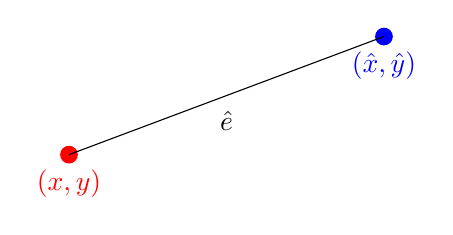
\begin{tikzpicture}
  \filldraw [red] (0,0) circle [radius=3pt] node[below=2pt] {$(x,y)$};
  \filldraw [blue] (4,1.5) circle [radius=3pt] node[below=2pt] {$(\hat{x},\hat{y})$};
  \draw (0,0) -- (4,1.5) node[midway,below=2pt] {$\hat{e}$};
\end{tikzpicture}
\end{center}

\begin{equation}
  \hat{e}(\hat{x},\hat{y})=\frac{1}{2}((x-\hat{x})^2+(y-\hat{y})^2)
\end{equation}

所以我们能够构造目标函数:
\begin{equation}
  f(\mathbf{x},\mathbf{y})=\sum^{5}_{i=1}\hat{e}_i
\end{equation}
\begin{eqnarray*}
\mathbf{x} & = &\left(x_1,x_2,x_3,x_4,x_5 \right)\\
\mathbf{y} & = & \left(y_1,y_2,y_3,y_4,y_5 \right)\\
\end{eqnarray*}

另外由于平面到成像平面的变换是一个射影变换,所以共线性不变,如下图所示,也就是说原本三点共线的几何性质不变(点1,点3,点5共线,点2,点4,点5共线),根据射影几何知识\cite{ref1},我们可以得到两个非线性等式约束。
\begin{eqnarray}
A_5^T\cdot (A_1\times A_3)&=&0\\
A_5^T\cdot (A_2\times A_4)&=&0
\end{eqnarray}

由公式(3),公式(4)可得约束公式:
\begin{eqnarray}
x_5y_1-x_5y_3+y_5x_3-y_5x_1+x_1y_3-y_1x_3&=&0\\
x_5y_2-x_5y_4+y_5x_4-y_5x_2+x_2y_4-y_2x_4&=&0
\end{eqnarray}
\begin{center}

\end{center}
因此公式(2),(5),(6)分别构成该最小二乘问题的目标函数和约束方程。

\begin{center}
\begin{tikzpicture}[scale=4,tdplot_main_coords]
  \coordinate (0) at (0,0,0);
  \coordinate (A3) at (0.3,0.8,0.3);
  \coordinate (A1) at (-0.5,0.9,0.6);
  \draw (A3) -- (A1);
  \coordinate (A5) at ($(A3)!.5!(A1)$);
  \draw[dashed,blue] (0) -- (A3);
  \node [fill=red,inner sep=1pt,label=right:$A_3'$] (A3n) at ($(0)!.5!(A3)$) {};
  \draw[dashed,blue] (0) -- (A5);
  \draw[dashed,blue] (0) -- (A1);
  \node [fill=red,inner sep=1pt,label=right:$A_1'$] (A1n) at ($(0)!4/9!(A1)$) {};
  \draw (A3n) -- (A1n);
  \node [fill=red,inner sep=1pt,label=right:$A_5'$] (A5n) at ($(0)!40/85!(A5)$) {};
  \node [fill=red,inner sep=2pt,label=right:$A_1$] (A1) at (A1) {};
  \node [fill=red,inner sep=2pt,label=right:$A_3$] (A3) at (A3) {};
  \node [fill=red,inner sep=2pt,label=right:$A_5$] (A5) at (A5) {};
  \draw[thick,->] (0,0,0) -- (1,0,0) node[anchor=north east]{$x$};
  \draw[thick,->] (0,0,0) -- (0,1,0) node[anchor=north west]{$y$};
  \draw[thick,->] (0,0,0) -- (0,0,1) node[anchor=south]{$z$};
  \draw (0.3,0.4,-0.2) -- (-0.4,0.4,-0.2) -- (-0.4,0.4,0.5) -- (0.3,0.4,0.5) -- (0.3,0.4,-0.2);
\end{tikzpicture}
\end{center}

\section{代码实现}
此处选用NLOPT工具\cite{ref2},经过多次测试,用Local derivative-free Constrained Optimization BY Linear Approximations\cite{ref3}\cite{ref4}优化算法来求解这个非线性约束问题能取得比较好的效果。NLOPT工具箱,其它算法可以参考\url{https://nlopt.readthedocs.io/en/latest/NLopt_Algorithms/}

\begin{lstlisting}[language=c++]
#include <iomanip>
#include <iostream>
#include <vector>
#include <nlopt.hpp>
#include <cstdio>

double myfunc(const std::vector<double> &x,
              std::vector<double> &grad,
              void *data)
{
  double *z = reinterpret_cast<double*> (data);
  if (!grad.empty())
  {
    grad[0] = - z[0] + x[0];
    grad[1] = - z[1] + x[1];
    grad[2] = - z[2] + x[2];
    grad[3] = - z[3] + x[3];
    grad[4] = - z[4] + x[4];
    grad[5] = - z[5] + x[5];
    grad[6] = - z[6] + x[6];
    grad[7] = - z[7] + x[7];
    grad[8] = - z[8] + x[8];
    grad[9] = - z[9] + x[9];
  }
  return (1/2.0 * ((z[0] - x[0])*(z[0] - x[0]) + (z[1] - x[1])*(z[1] -x[1]) + (z[2] - x[2])*(z[2] - x[2]) + (z[3] - x[3])*(z[3] - x[3]) + (z[4] - x[4])*(z[4] - x[4]) + (z[5] - x[5])*(z[5] - x[5]) + (z[6] - x[6])*(z[6] - x[6]) + (z[7] - x[7])*(z[7] - x[7]) + (z[8] - x[8])*(z[8] - x[8]) + (z[9] - x[9])*(z[9] - x[9])));
}

double myconstraint1(const std::vector<double> &x,
                     std::vector<double> &grad,
                     void *data)
{
  if (!grad.empty())
  {
    grad[0] = 0.0;
    grad[1] = 0.0;
    grad[2] = x[7] - x[9];
    grad[3] = x[8] - x[6];
    grad[4] = 0.0;
    grad[5] = 0.0;
    grad[6] = x[9] - x[3];
    grad[7] = x[2] - x[8];
    grad[8] = x[3] - x[7];
    grad[9] = x[6] - x[2];
  }
  printf("constraint1 = %g\n", (x[8]*x[3] - x[8]*x[7] + x[9]*x[6] - x[9]*x[2] + x[2]*x[7] - x[3]*x[6]));
  return (x[8]*x[3] - x[8]*x[7] + x[9]*x[6] - x[9]*x[2] + x[2]*x[7] - x[3]*x[6]);
}

double myconstraint2(const std::vector<double> &x,
                     std::vector<double> &grad,
                     void *data)
{
  if (!grad.empty())
  {
    grad[0] = x[5] - x[9];
    grad[1] = x[8] - x[4];
    grad[2] = 0.0;
    grad[3] = 0.0;
    grad[4] = x[9] - x[1];
    grad[5] = x[0] - x[9];
    grad[6] = 0.0;
    grad[7] = 0.0;
    grad[8] = x[1] - x[5];
    grad[9] = x[4] - x[0];
  }
  printf("constraint2 = %g\n", (x[8]*x[1] - x[8]*x[5] + x[9]*x[4] - x[9]*x[0] + x[0]*x[5] - x[1]*x[4]));
  return (x[8]*x[1] - x[8]*x[5] + x[9]*x[4] - x[9]*x[0] + x[0]*x[5] - x[1]*x[4]);
}

std::vector<double> led_nlopt(double *data)
{
  nlopt::opt opt(nlopt::LN_COBYLA, 10);

  opt.set_lower_bounds(0.0);
  opt.set_upper_bounds(128.0);

  opt.set_min_objective(myfunc, data);
  opt.add_equality_constraint(myconstraint1, NULL, 1e-8); 
  opt.add_equality_constraint(myconstraint2, NULL, 1e-8);
  opt.set_xtol_rel(1e-8);

  double minf;
  int count = 0;
  std::vector<double> x(10);
  x.assign(&data[0],&data[10]);

  /*std::cout << data << "\n" << &x << std::endl;*/
  try{
    nlopt::result result = opt.optimize(x, minf);
  }
  catch(std::exception &e) {
    std::cout << "nlopt failed" << e.what() << std::endl;
  }

  return x;
}


int main(int argc, char* argv[])
{
  double led_posi[10] = { 105.17, 22.84, 104.49, 59.80, 68.70, 58.41, 69.34, 21.42, 86.22, 39.48};

  std::vector<double> x = led_nlopt(led_posi);
  
  printf("%0.10g, %0.10g, %0.10g, %0.10g, %0.10g, %0.10g, %0.10g, %0.10g, %0.10g, %0.10g\n", 
	x[0], x[1], x[2], x[3], x[4], x[5], x[6], x[7], x[8], x[9]);

  return 0;
}
\end{lstlisting}
输出结果:
\begin{lstlisting}
constraint1 = 0
constraint2 = 4.09273e-12
104.8604201, 22.52263159, 104.557343, 59.73833188, 68.392894, 58.09516744, 69.40955282,
 21.35630824, 86.69979044, 40.23756096
\end{lstlisting}
\section{总结}
在现有的检测算法里常常会出现检测点偏差过大,导致检测到的平台形状不能很好匹配实际平台的形状。于是通过加入额外多余的一个点去检测测量结果,形成两个约束去弱化这种现象。该方法需要注意的地方是优化前一定要{\color{red}{注意匹配好点的位置}}。另外这个方法只能保证检测到的点的几何关系,并不能保证点的位置,解决方法可以通过调整目标函数里的权重去解决。

\begin{thebibliography}{99}  
\bibitem{ref1}Richard Hartley, Andrew Zisserman, Tian L, "Multiple View Geometry in Computer Vision." (2000), Page 27-28. 
\bibitem{ref2}Steven G. Johnson, The NLopt nonlinear-optimization package, http://ab-initio.mit.edu/nlopt.
\bibitem{ref3}M. J. D. Powell, "A direct search optimization method that models the objective and constraint functions by linear interpolation," in Advances in Optimization and Numerical Analysis, eds. S. Gomez and J.-P. Hennart (Kluwer Academic: Dordrecht, 1994), p. 51-67.
\bibitem{ref4}M. J. D. Powell, "Direct search algorithms for optimization calculations," Acta Numerica 7, 287-336 (1998).
 
\end{thebibliography}

\end{CJK*}
\end{document}